\chapter{Architecture}

This chapter provides an overview of the architecture for the hashing
accelerator and the DMA module designed in the project.

\section{Design of the Hashing Accelerator}

As noted in section \ref{sec:previous-hash}, there are many options for
designing a hashing module. Searching the internet, several open-source
implementations of such modules can be found. However, most of these
take advantage of various optimizations which makes the code hard to
read or unsuitable for use in an FPGA.

It was decided to create a new hashing module, using optimizations only
if neccessary, focusing on creating well-written and easy-to-read source
code that can later be easily extended or modified.

To do this, a simple module was constructed that runs one iteration of
the compression function each cycle, calculating the hash of one block
of data in 64 cycles with one additional cycle added for creating the
final hash from the intermediate values from the previous round (see
section \ref{sec:hashing-algo} for details).

Using no optimizations yielded a hashing accelerator module that can
run at 50~MHz, the same clock frequency as used in the SHMAC system.
Because of this, and in order to preserve the readability of the code, it
was decided not to attempt to improve the performance of the module.

\subsection{Theoretical Maximum Performance}
If the hashing module can finish hashing a block of data in 65 cycles and
every hash can be obtained from only one block of data, it is possible to
obtain a finished hash every 65 clock cycles under ideal conditions. This
translates into a maximum theoretical performance of 768230~H/s at a clock
frequency of 50~MHz.

However, in real-life, the modules do not exist in a vacuum, and data needs to be transferred
between the modules and a controller, such as a microprocessor. If the hashing tiles
are connected to the rest of the system using an AXI4 lite interface, transfers
takes at least three cycles for writes and two cycles for reads.
It is assumed that no burst transfers are used and that only one transaction
can be executed at a time, corresponding with the requirements for the interface.

In order for the hashing module to work, it needs 16 32-bit words of input data,
and control signals must be set up. This causes at least 17 words of data to
need to be written to the module, taking at least 51 clock cycles. Then, after
hashing of a block is complete, if there are no more blocks, the result must
be read back. The result consists of 8 words of data, which takes at least 16
clock cycles to transfer.

In total, a minimum of 67 clock cycles of overhead is needed per hash when assuming
a one-block input size and an ideal AXI4 bus. Not considering the additional overhead
from processing in the microprocessor, such as when handlig the interrupt when the
hashing finishes, hashing may take a minimum of $67 + 65 = 132$ clock cycles to
complete, bringing the maximum theoretical performance down to at most 378787~H/s.

\section{Design of the DMA Module}
\label{sec:dma-architecture}

\subsection{Assumptions}
To simplify the design of the DMA module, some assumptions as to the system where the
DMA is implemented needs to be done.

It is assumed that all data is transferred sequentially. 
This is especially important when it comes to future integration into the SHMAC system, because of the XY routing that the system uses.
However, such an assumption also significantly simplifies the design of the DMA for use in shared-bus systems.

Virtual memory and cache coherency are assumed to be handled outside the \todo{and therefore not in the project. Mention?} DMA module.

%\subsection{Design requirements}
\subsection{Chosen functionality in design}

It was decided on a couple of requirements for the DMA implementation.

\begin{description}
	\item[Use block-to-block transfers.] This is a minimum requirement for being
	able to transfer any amount of data from location A to B.
	\item[Two channels.] This allows the DMA to have two separate transfers going
	at the same time.
	The number of channels is inspired by the Adapteva Epiphany \cite{epiphany}, where every DMA module has two generic channel each.
	With a high number of DMA modules, a high number of channels in each DMA module is not necessary.
	\todo{This was actually not a requirement, and I think of describing it in State Machine. Consider removal}\item[Automatic channel allocation.] Channel allocation is done in hardware,
	saving the CPU from the overhead of allocating and managing channels in software.
	% I removed component-based implementation, because _every_ hardware design is component based. -K.
	% 
	% Yeah.... that makes sense. You should have taken TFE4140 last spring, not every student though of component based design, as they threw together a lot of code at top-level :-P
\end{description}

\subsection{DMA Architecture}

The DMA module consists of several main components: a FIFO buffer that contains transfer
requests from the CPU, a main controller that processes the requests, and two channels
where the memory transfers are executed. The two channels work on independent transfer
tasks. An arbiter is used to control access to the bus interface for the two channels.
An overview of the DMA architecture can be seen in figure \ref{fig:DMATopView2}.
\todo{CNTR = counter --- CTRL = controller, please fix the figure}
The overview provided in this chapter is simplified.
For more details, see appendix \todo{Yep!} INSERT REF HERE, FIND OUT HOW TO DO SEC-LABEL

\begin{figure}[htb]
    \centering
    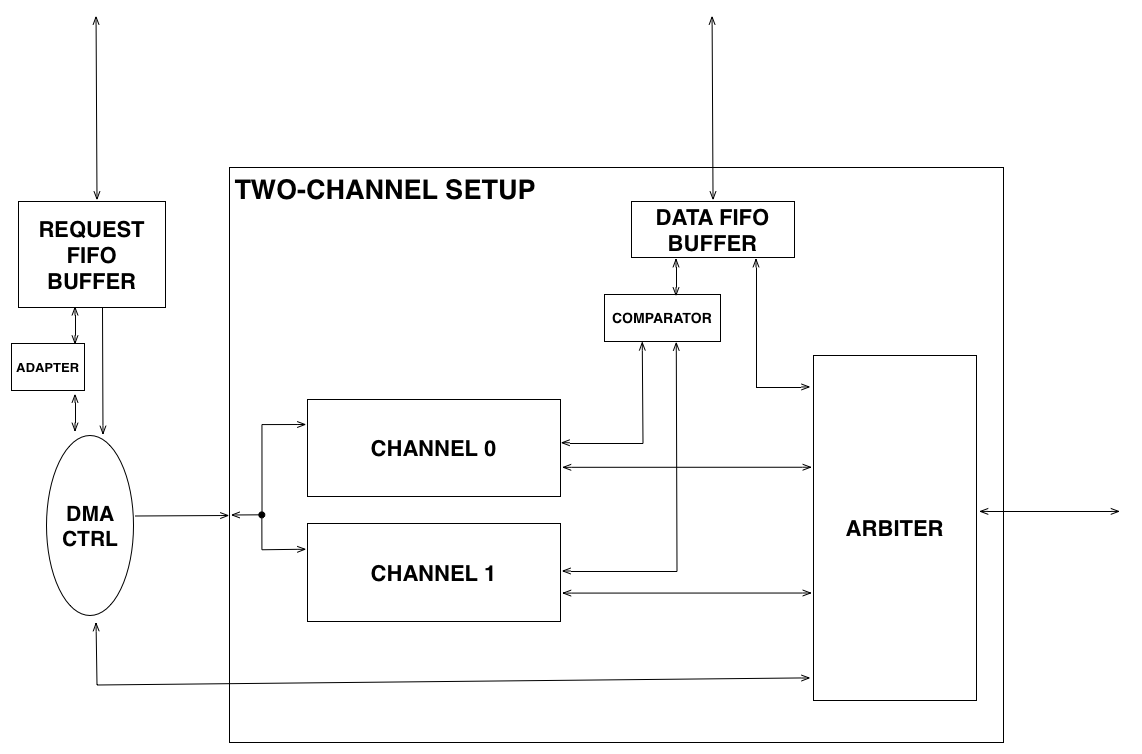
\includegraphics[width=1\textwidth]{Figures/DMA/TopViewFinalSimple2}
    \caption{DMA module overview}
    \label{fig:DMATopView2}
\end{figure}

\subsubsection{Main Controller}
The role of the main controller is to process incoming transfer requests, allocate and activate
channels that are free to execute requests, monitor the channels, and send out an interrupt signal
when a transfer is completed.

The controller is implemented as a state machine, shown in figure \ref{fig:DMAControllerStateMachineSimple}.

\begin{figure}[htb]
    \centering
    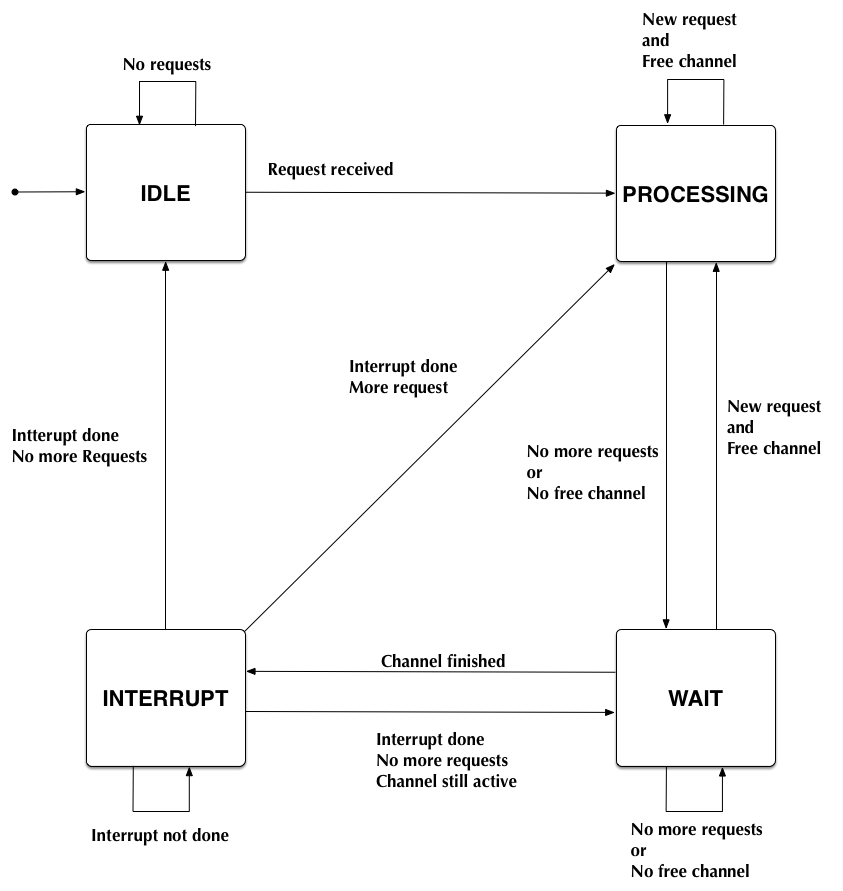
\includegraphics[width=1\textwidth]{Figures/DMA/StateMachineFinalSimple}
    \caption{DMA Controller State Machine}
    \label{fig:DMAControllerStateMachineSimple2}
\end{figure}

% IMPORTANT: Before you start talking about being too detailed, Kristian, my group got slaugthered in Computer Architecture project (TDT4260) for showing figures in result section without explaining them in the text. Do not count on figures to be self-explanatory. 
Four states are used: IDLE; PROCESSING, WAIT and INTERRUPT.
Whenever there is no activity and no incoming tranfer request, the state is IDLE.
When activating a new channel for a requested transfer, the state is PROCESSING. There must be a request to handle, and at least a free channel to jump to this state from any other state.
When at least one channel is active, the state is WAIT as long as no more channels can be activated (either due to no more requests or all channels already being active).
When sending out interrupt signal, the state is INTERRUPT.

\subsubsection{Channels}
A channel is split into two parts: a part that is responsible for sending out load
commands, and a storing part that issues a store commands. These ``subchannels''
are called the load channel and store channel, respectively.
The load channel will send out requests for loading data as long as its counter indicates that there is more data to be loaded. The store channel will request stores only when the loaded data is ready in the Data FIFO buffer.
Each of these contains registers for calculating source addresses, destination addresses and for counters.
\todo{Perhaps add an overview picture of channels here}

\subsubsection{FIFO buffers}
Two FIFO (First-In-First-Out) buffers are used in storing incoming transfer requests for the DMA Controller, and for storing incoming data loaded by the channels.
The choice in using FIFO buffers are to enable the DMA module to be implemented in systems where multiple requests or multiple datas may arrive before any is handled.

\subsubsection{Arbiter}
The arbiter arbitrates between the channels and the DMA Controller.
Whenever any channel or the Controller request to send through data (addresses for loading/storing, data for storing or interrupt details), the arbiter must select one of these requests.
The request will be acknowledged, and the data sent through.
Interrupt requests have highest priority, followed by storing requests and then loading requests.
The requesting DMA Controller or channel is updated when acknowledged (either ending INTERRUPT state, or decrementing a channel counter).

\subsubsection{Comparator}
This is simple combinatorics, used to compare expected data from all store channels with next ready data.
Whenever there is a match, the correct store channel is notified, so that it can request storing the data with the destination address calculated from the channel.

\subsubsection{Bus interaction system}
In order for the DMA module to be as general as possible, it contains only a generic
interface for communicating with a bus system. An adapter is then used to connect
the module to the bus system. This makes it possible to connect the DMA module to
different kinds of busses by simply writing an adapter for the desired system.


\section{Alternative Simplified Designs} 
\todo{Yaman told us to move this kind of discussion to the end of the report}
In order for the design to be more appropriate for environments where there are
constraints on, for example, logic resources or size of the module, certain simplifications
are possible.

\todo{Consider making diagrams to show the alternatives}

\subsection{Reducing the Controller Logic}
It is possible to remove some of the main components from the DMA module and still
have a functional DMA module. The request FIFO and the DMA controller could be removed,
and a channel could be directly connected to the bus interface adapter with little
extra work.

This would slightly reduce the number of cycles that is needed to process a request.
The system would also be smaller, including less combinatorics and registers.

On the other hand, this makes the DMA module much more dependent on the external system, since requests are processed and set externally, not by the DMA module itself.
Futhermore, removing the controller also constricts the possibility for the DMA module itself to be able to process different types of requests.
In the minimum case, the only requests that it needs to handle are data transfer requests.
But if the DMA module is implemented in the SHMAC system, and one wants an as efficient data transfer as possible, one have to consider the option of dynamicly forwarding the request.
An example would be forwarding to the DMA module that is \todo{Mentioned in chapter 3.5.1., see figure 3.3} closest to both source and destination.

Part of the purpose with the design is to make the DMA module generic, so that it can implemented in different systems.
In order to make the design as generic as possible, a controller and an incoming request FIFO
in case of multiple requests is therefore essential.

\subsection{Using Channels with a Private Data Buffer}
Instead of using a channel with shared data buffer, where the data output owned by
one of the channels is sent straight through the arbiter, it could be sent to a
private buffer inside the correct channel.
\todo{An explanation of the shared/private buffers will need to be added somewhere}

\todo{Expand when you wake up from bed. Good night}
Pros: Secure data

Cons: More unnecessary combinatorics + no better throughput

